%-------------------------------------------------------------------------------
%-------------------------------------------------------------------------------
\begin{frame} I heavily draw on the material presented in:

\begin{itemize}
\item \bibentry{Lee.2010a}
\end{itemize}

\end{frame}
%-------------------------------------------------------------------------------
%-------------------------------------------------------------------------------
\begin{frame}\textbf{Issues}\vspace{0.3cm}
\begin{itemize}\setlength\itemsep{1em}
\item intuition
\item identification
\item interpretation
\item estimation
\end{itemize}

\end{frame}
%-------------------------------------------------------------------------------
%-------------------------------------------------------------------------------
\begin{frame}\textbf{Key points}\vspace{0.3cm}

\begin{itemize}\setlength\itemsep{1em}
\item RD designs can be invalid if individuals can precisely manipulate the assignment variable.
  \begin{itemize}\medskip
  \item discontinuity rules might generate incentives
  \end{itemize}
\item If individuals - even while having some influence - are unable to \textbf{precisely} manipulate the assignment variable, a \textbf{consequence} of this is that the variation in treatment near the threshold is randomized as though from a randomized experiment.
  \begin{itemize}\medskip
  \item contrast to IV assumption
  \end{itemize}
\end{itemize}
\end{frame}
%-------------------------------------------------------------------------------
%-------------------------------------------------------------------------------
\begin{frame}\textbf{Key points}\vspace{0.3cm}

\begin{itemize}\setlength\itemsep{1em}
\item RD designs can be analyzed - and tested - like randomized experiments.
\item Graphical representation of an RD design is helpful and informative, but the visual presentation should not be tilted toward either finding an effect or finding no effect.
\item Nonparametric estimation does not represent a "solution" to functional form issues raised by RD designs. It is therefore helpful to view it as a complement to - rather than a substitute for - parametric estimation.
\end{itemize}

\end{frame}
%-------------------------------------------------------------------------------
%-------------------------------------------------------------------------------
\begin{frame}\textbf{Key points}\vspace{0.3cm}

\begin{itemize}\setlength\itemsep{1em}
\item Goodness-of-fit and other statistical tests can help rule out overly restrictive specifications.
\end{itemize}

\end{frame}
%-------------------------------------------------------------------------------
%-------------------------------------------------------------------------------
\begin{frame}\textbf{Baseline}\vspace{0.3cm}

A simple way to estimating the treatment effect $\tau$ is to run the following linear regression.
%
\begin{align*}
Y = \alpha + D \tau + X \beta + \epsilon,
\end{align*}
where $D \in [0, 1]$ and we have $D = 1$ if $X \geq c$ and $D=0$ otherwise.
\end{frame}
%-------------------------------------------------------------------------------
%-------------------------------------------------------------------------------
\begin{frame}\textbf{Baseline setup}\vspace{0.3cm}

\begin{figure}[htp]\centering
\scalebox{0.60}{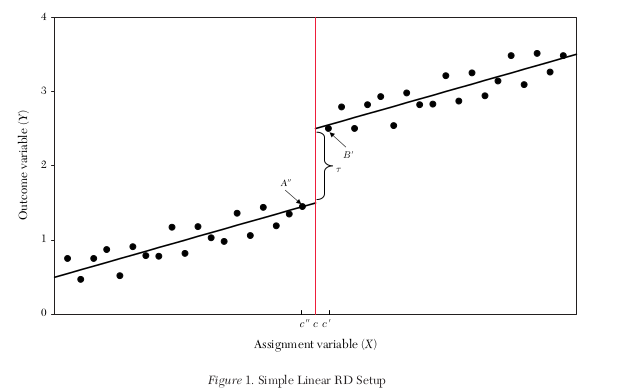
\includegraphics{material/fig-1}}
\end{figure}

\end{frame}
%-------------------------------------------------------------------------------
%-------------------------------------------------------------------------------
\begin{frame}\textbf{Potential outcome framework}\vspace{0.3cm}

\begin{figure}[htp]\centering
\scalebox{0.60}{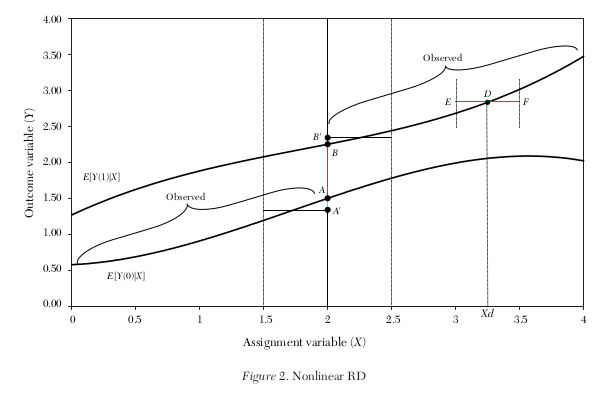
\includegraphics{material/fig-2}}
\end{figure}

\end{frame}
%-------------------------------------------------------------------------------
%-------------------------------------------------------------------------------
\begin{frame}\textbf{Potential outcome framework}

\begin{align*}
E[Y_i(1) - Y_i(0) \mid X = c]
\end{align*}
$\Rightarrow$ average treatment effect at the cutoff

\end{frame}
%-------------------------------------------------------------------------------
%-------------------------------------------------------------------------------
\begin{frame}\textbf{Alternatives}\vspace{0.3cm}

Consider the standard assumptions for matching:\vspace{0.3cm}

\begin{itemize}\setlength\itemsep{1em}
\item ignorability\medskip
  \begin{itemize}
  \item trivially satisfied by research design
  \end{itemize}
\item common support\medskip
  \begin{itemize}
  \item cannot be satisfied and replaced by continuity
  \end{itemize}
\end{itemize}


\end{frame}
%-------------------------------------------------------------------------------
%-------------------------------------------------------------------------------
\begin{frame}\textbf{Alternatives}\vspace{0.3cm}

\citeA{Lee.2010a} emphasize the close connection of RDD to randomized experiments.\vspace{0.3cm}

\begin{itemize}
\item How does the graph in the potential outcome framework change?
\end{itemize}

\end{frame}
%-------------------------------------------------------------------------------
%-------------------------------------------------------------------------------
\begin{frame}

\begin{figure}[htp]\centering
\scalebox{0.60}{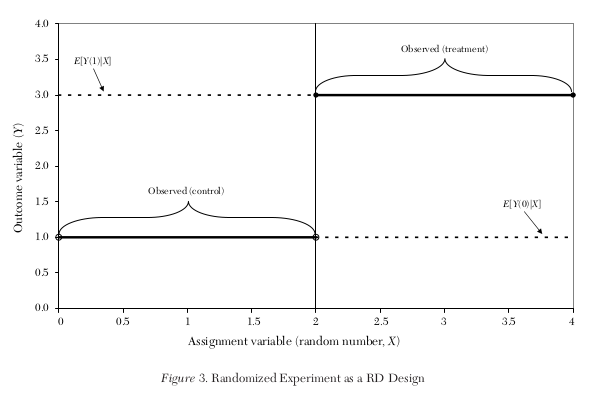
\includegraphics{material/fig-3}}
\end{figure}

\end{frame}
%-------------------------------------------------------------------------------
%-------------------------------------------------------------------------------
\begin{frame}

\begin{itemize}
\item \textit{Continuity}, the key assumption of RDD, is a \textbf{consequence} of the research design and not simply imposed.

\end{itemize}

\end{frame}
